%   Version 4.1r of REVTeX, August 2010
%
%   Copyright (c) 2009, 2010 The American Physical Society.
%
%   See the REVTeX 4 README file for restrictions and more information.
%
% TeX'ing this file requires that you have AMS-LaTeX 2.0 installed
% as well as the rest of the prerequisites for REVTeX 4.1
%
% See the REVTeX 4 README file
% It also requires running BibTeX. The commands are as follows:
%
%  1)  latex apssamp.tex
%  2)  bibtex apssamp
%  3)  latex apssamp.tex
%  4)  latex apssamp.tex
%

\documentclass[%
twocolumn,
%superscriptaddress,
%groupedaddress,
%unsortedaddress,2
%runinaddress,
%frontmatterverbose, 
%preprint,
%showpacs,preprintnumbers,
%nofootinbib,
%nobibnotes,
%bibnotes,
 amsmath,amssymb,
 aps, citeautoscript,
%pra,
prb,
%rmp,
%prstab,
%prstper,
%floatfix,
]{revtex4-1}

\usepackage{graphicx}% Include figure files
\usepackage{dcolumn}% Align table columns on decimal point
\usepackage{bm}% bold math

%\usepackage{hyperref}% add hypertext capabilities
%\usepackage[mathlines]{lineno}% Enable numbering of text and display math
%\linenumbers\relax % Commence numbering lines

%\usepackage[showframe,%Uncomment any one of the following lines to test 
%%scale=0.7, marginratio={1:1, 2:3}, ignoreall,% default settings
%%text={7in,10in},centering,
%%margin=1.5in,
%%total={6.5in,8.75in}, top=1.2in, left=0.9in, includefoot,
%%height=10in,a5paper,hmargin={3cm,0.8in},
%]{geometry}

\begin{document}

\preprint{APS/123-QED}

\title{Predicting band gap correction for perovskite oxide using high throughput and machine learning}% Force line breaks with \\
%\thanks{A footnote to the article title}%

\author{Wei Li}
\affiliation{Department of Materials Science and Engineering, University of Delaware, Newark, DE 19716, USA}
\author{Zigeng Wang}
\affiliation{Computer Science and Engineering Department, University of Connecticut, USA,19716, USA}
\author{Xia Xiao}
\affiliation{Computer Science and Engineering Department, University of Connecticut, USA,19716, USA}
\author{Zhiqiang Zhang}
\affiliation{Department of Physics, University of Delaware, Newark, DE 19716, USA}
\author{Rajasekaran, Sanguthevar}
\affiliation{Computer Science and Engineering Department, University of Connecticut, USA,19716, USA}
\author{Bharat Medasani}
\affiliation{Delaware Energy Institute, University of Delaware, Newark, DE 19702, USA}
\author{Anderson Janotti}
\affiliation{Department of Materials Science and Engineering, University of Delaware, Newark, DE 19716, USA}
\email{janotti@udel.edu}

\date{\today}% It is always \today, today,
             %  but any date may be explicitly specified
\begin{abstract}

Recent advances in computing power have enabled the generation of large datasets for materials, enabling data-driven approaches to problem-solving in materials science, including materials discovery. Machine learning is a primary tool for manipulating such large datasets, predicting unknown material properties and uncovering relationships between structure and property. A machine learning model is developed that can accurately predict the HSE06 band gap correction to the PBEsol level of pervoskite oxide family compounds by -0.145 eV, by quantitatively analyzing the valence band maximum (VBM) and conduction band minimum (CBM) offset. Not only does this resulting tool provide the ability to accurately predict the HSE06 band gap based on the PBEsol results but also the speed of the prediction based only on the cubic structure will make this a great resource to screen functional pervoskite materials. And this design represents a powerful database and tool for mapping the vast materials landscape and accelerating discovery. 


%\begin{description}
%\item[Key words]
%Secondary publications and information retrieval purposes.
%\end{description}
\end{abstract}

%\pacs{Valid PACS appear here}% PACS, the Physics and Astronomy
                             % Classification Scheme.
%\keywords{Suggested keywords}%Use showkeys class option if keyword
                              %display desired
\maketitle

%\tableofcontents

\section{Introduction}
 
Density functional theory (DFT) is often used to predict crystal structure lattice parameters, within 1-2 of the experimental values and the scalability of computations makes it possible to make predictions on thousands of materials.  However, there is a systematic under-estimation of the band gap, E$_g$, compared with the experimental values when employing standard exchange and correlation functionals such as the generalized gradient approximation as proposed by Perdew, Burke, and Ernzerhof (PBE) [1].  Hybrid functionals  [2,3] or the Green’s function quasi-particle GW methods  [4,5] improve accuracy, yet are much more expensive computationally, precluding their systematic use in searching over thousands of compounds. To accelerate the discovery and development of new materials for electronic and optoelectronic applications, it is desirable to have an automating and scaling computational approach that predicts accurate values for band gaps at the speed or faster than DFT-PBE calculations. Over the last decade, ML has been applied to materials science problems in a variety of directions, such as prediction and classification of crystal structures, development of interatomic potentials,18,19,20 finding of optimal density functionals for density functional theory, and building of predictive models of material properties. Several research groups have demonstrated the benefits of automating and scaling computational property. For example, an overview of high-throughput band structure calculations by Curtarolo et al. [6] New materials for radiation detectors is suggested by screening about 22,000 materials by Hachmann, et al. [7]

Instead of the conventional computational materials design, which derived materials properties according to physical law, for example, solving the Kohn-Sham equation, ML can learn the hidden rules based on a large data set and build a model to make corresponding predictions. So far, the main data for perovskite formability can be found in a few articles(ref 8-11) that summarized the existing experimental data and prevalent databases. The statistical learning has emerged as a promising tool for predicting the cohesive energy, lattice thermal conductivity, band gaps, free energy, and heat capacity within reasonable time. 

\begin{figure}[ht!]
\begin{center}
\includegraphics[width=3.6 in]{Figures/Fig1.eps}
\end{center}
\caption{ Crystal structures of garnet and perovskite prototypes.Green, blue and red spheres are atoms of A, B and X sites, respectively. a crystal structrure of $pm3^{bar}m$ cubic structure. b crystal structure of $I4_mmm$ tetragonal structure. c crystal structure of $Pnma$ orthohombic structure.}
\label{fig1}
\end{figure}

Our project is designed to develop a database of calculated material properties and enable accelerated materials discovery by machine learning approach on the functional inorganic materials, which are used in applications such as LEDs  [8,9], transistors[8]  and solar cells  [10]with specific band gaps, starting with perovskite class of materials. An attractive feature of perovskite class of materials with a formula of ABX3, where X is  typically  oxygen,  is  the  possibility  of  tailoring  their  band  gaps  by changing the elemental composition of the A, B, and/or X sites, as well as possible rotations and tilting of the BX6 octahedra.  It is therefore of high technological interest to explore all possible perovskite materials with desirable electronic properties for optoelectronic applications.   

In this project we are developing a machine learning models as Fig.1 for mapping DFT-PBE computed band gaps of perovskites into experimental band gaps.  This will enable us to provide high fidelity band gaps without a significant increase in computational cost.  To generate DFT based observables and reliable database, we are calculating DFT bandgaps via high-throughput approach and find out the band gap correction and band offset between two approximations. Later on, we plan to extend this approach to explore the electronic structure of chalcogenides, and halides.  The machine learning models helps us in gaining a fundamental understanding of the most relevant factors of the elements, such as atomic orbital energies, interatomic distances, etc, in the determination of band gaps. We believe that this type of crude estimations of properties can be interesting supplement to standard features.  This crude estimation of properties consists of the calculation of a target property (the experiment band gap) utilizing crude estimators (the calculated PBEsol band gap). This machine learning algorithm no longer needs to predict a target property but rather an correction or a difference between properties calculated with two well-defined methodologies. 

\section{Method and computational details}

First-printciples calculations based on DFT are carried out based on the Vienna ab initio simulation packaged with plane-wave pseudopotential method\cite{}. The wave functions are expaned in the plane wave up to a cutoff energy of 650 eV. The exchange-correlation function we used in the general approximation of Perdew, Burke and Drnzernhof\cite{}. The Brillouin zones were diveded by Monckhorst Pack k-mesh with 6X6X6, ..... grid in the case of cubic, tetragonal and orthorhombic structure optimization and electronic structure calculations.
The learning model is developed for the given band gap data set {X, y}, which maps input feature set X to the targeted HSE band gap y. Here, X = ${x_{i}}_{i = 1} ^{n}$ consists of $n$ individual features (with $n$ = 4). These relevant features are selected by the regression technique ( XGBoost ) and reduced to in the feature set. 


A data set comprising ~400 perovskite was generated by performing the full DFT relaxation and energy calculations on all allowed species on the A, B sites.  
To build the learnign model, {X, y} is split into the training, testing and validation sets in the ratio of 80:15:5.  

\begin{figure}[ht!]
\begin{center}
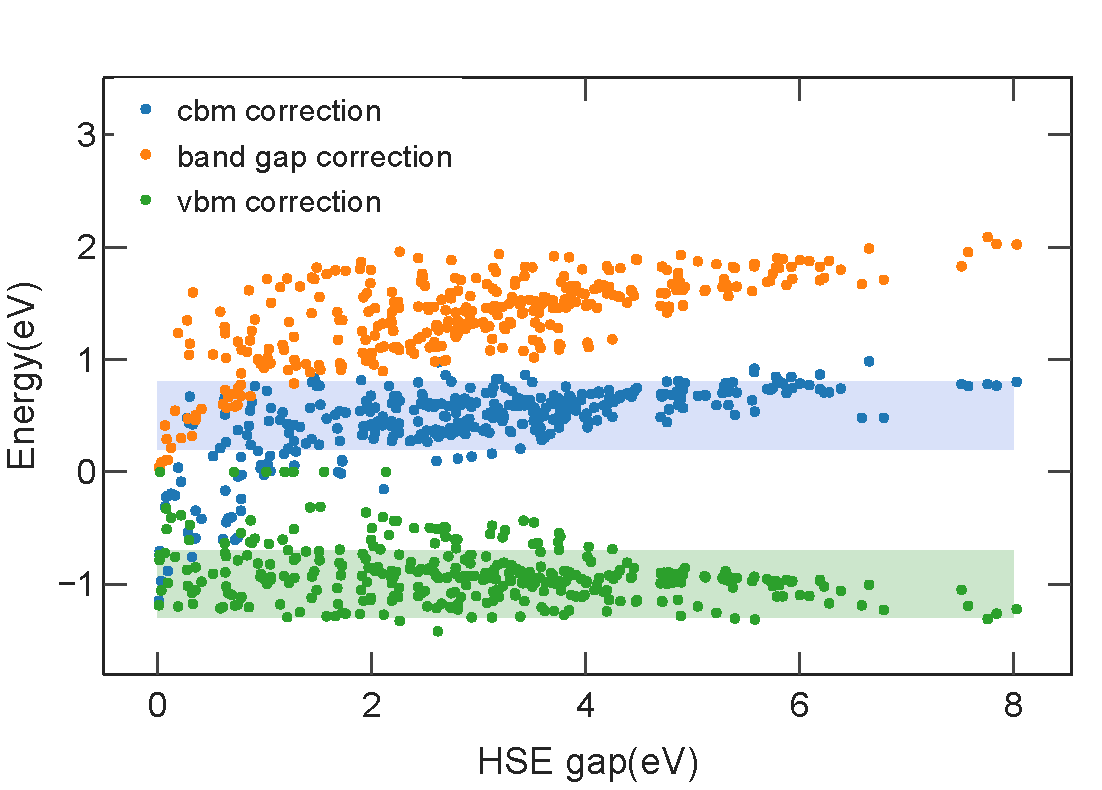
\includegraphics[width=3.0in]{Figures/Fig2.pdf}
\end{center}
\caption{ The HSE06 functional correction comparing with PBEsol functional for the band gap (orangle), VBM offset(green) and CBM offset(blue) for (a) cubic structure, (b) tetragonal structure, (c) orthorhombic structure. 
}
\label{fig1}
\end{figure}

\begin{figure*}[ht!]
\begin{center}
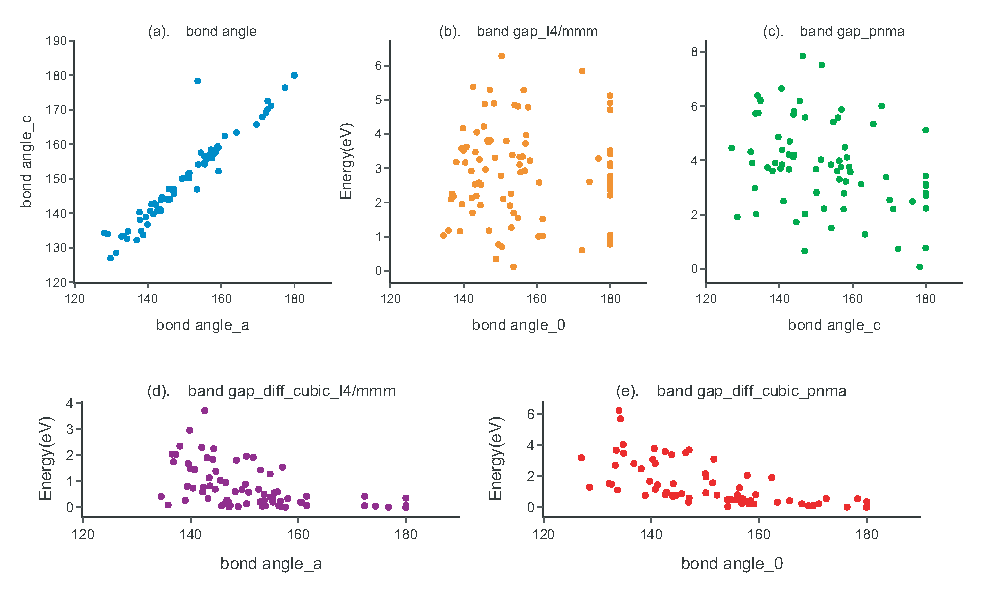
\includegraphics[width=6.0in]{Figures/Fig3.eps}
\end{center}
\caption{ (a) the correlation functional relationship between the equatorial and apical bond angle in the orthorhombic structure (space group $Pnma$).
(b) The DFT band gap of the tetragonal structure (space group $I4_mmm$) as a function of the apical B-O-B bond angles. 
(c) Two-dimensional map of the DFT band gap of the orthorhombic structure as a function of the apical B-O-B bond angles. 
(e) The map of the DFT band gap difference between cubic structure and tetragonal structure. 
(e) The map of the DFT band gap difference between cubic structure and orthorhombic structure. 
}
\label{fig1}
\end{figure*}


\section{Results and Discussions}

We are filtering the perovskite space such that the selected A and B chosen to give semiconducting materials, i.e., valence(A)+valence(B)=6, which totally comes with 118 formulas.
For each compound, four common phases, as shown in Figure 1, are considered. Those four space groups dominate the crystal structure of existing oxides $ABO_{3}$ compounds. Cubic phase is the ideal perovskite structure without distortion, as shown in Fig.1(a). By considering 118 compounds with four crystal phase, we have a total of 590 systems of interest for further study.
. With octahedral rotation and different phase, approximately 1000 materials will be used in our analyze at the beginning, and it will involve more materials later on.

We developed an ...(   ) model for intrinsic perovskite with a data set comprising compounds which were generated by performing full DFT relaxation and non self-consistent calculations on all combinations of allowed species(Supplementary Table ..) on the A and B site. This dataset was randomly divided into training, validation and test data in the ration of (7:2:1). We find that this architecture yields a small root mean square error(RMSE) of ? eV, as well as the smallest standard deviation ... For comparison, the error in the DFT Eg of perovskite relative to experimental values is around ? eV.   
a
The systematic underestimation of DFT with standard exchange and correlation functional such as LDA or PBE/PBEsol stems from the well-known discontinuity in the derivative of exchange and correlation functional as the number of electrons deviates from integers. Indeed, PBE deviates from the expected straight-line behavior between two integer charges following a convex curvature, referred to as self-interaction. This self-interaction leads to erroneous localization and tends to spread the charges across a system. Hartree-Fock, on the contrary, shows a concave behavior for many-electron systems, resulting in localization of charges. A hybrid exchange and correlation function , which mixes a fracction of PBE with a fraction of Hartree-Fock, produces the almost straight-line behavior, as desired. The band gaps calculated using hybrid funcitonals show excellent agreement with the experimental results. However, using hybrid fucntionals increases the computational cost by several orders of magnitude compared with PBE. 

This machine learning algorithm shows that we can predict HSE06 functional band gaps trained using the E$_{gPBE}$ values. 

Previous theoretical calculations revealed that the lattice distortion does not significantly impact the electronic and optical properties of the halide perovskite, but B-X bond breaking with face-shared or line-shared octahedral can destroy the unique properties of perovskites.

Fig 2. Indicating that the VBM position falls approximately -1 eV from PBEsol functional and the hybrid functional. Among the selected compounds, the only place perform poorly is in the family of Cu, Pb, Sn as A site and TL as B site with VBM falls larger than -0.75 eV.
However, the error in this case is still only \%20 with a predicted value. The deviation for VBM is not surprising considering that Cu, Pb and Sn family have higher d orbital energy than oxigen 2p orbital. 

Fig 3. (a) is the map between the apical bond angle and equatorial bond angle in the $Pnma$ structure. It shows a linear function with apical bond angle $\approx$ equatorial bond angle, which is a correction() for the ref\cite{} investigation. 

Based on our Fig 3.(b) and (c), there is no specific correlation between the DFT band gap and the B-O-B bond angle in the structure. We shows singnificant scatter data dispersion at all the range of the B-O-B bond angle when we change the AB combination. 

One interesting comparison is the band gap relationship between the cubic (pm$3_bar$m) structure and tetragonal($I4mmm$)\& orthombhedral$pnma$ structure. With octahedral rotation, the band gap not surprisingly increase but always less than 1 eV as shown in Fig3 (d) and (e). 

\section{Summary}

In summary, this contribution presents a supervised machine-learning scheme trained using 100 DFT calculated band gaps. Our results show that this method, using a descriptor set based on only composition information, is capable of determination HSE06 functional band gaps, valence band maximum (VBM) and conduction band minimum (CBM) offset with PBEsol functional. 
These results are significant because they present an model that can reliably predict the band gap at a drastically reduced computational cost compared with higher levels of theory.
While this method does not directly correct the PBE band gap for the self-interaction term, it is a powerful way to map computationally cheap methods such as PBEsol to relatively expensive methods such as HSE through finding out the band correction on a specific family compounds. Expansion of this work to other family compounds could enable NNs to augment traditional DFT methods to both lower computational costs and increase accuracy. 
Finally, the success of this method enables us to employ our model to estimate the band gap of other compounds 

\section{Data availability}

The datasets generated during and/or analysed during the current study are available in
the GitHub repository https://github.com/ as well as the
Dryad Digital Repository (doi: 10.5061/). A web application that estimates Eg 

\section{Acknowledgments}

This work was supported by the National Science Foundation Faculty Early Career Development Program DMR-1652994. This research was also supported by the the eXtreme Science and Engineering Discovery Environment (XSEDE) facility, National Science Foundation grant number ACI-1053575, and the Information Technologies (IT) resources at the University of Delaware, specifically the high performance computing resources.

\bibliography{BIB}

\end{document}